
%(BEGIN_QUESTION)
% Copyright 2014, Tony R. Kuphaldt, released under the Creative Commons Attribution License (v 1.0)
% This means you may do almost anything with this work of mine, so long as you give me proper credit

Determine all component voltages and currents in this circuit, being sure to mark directions of all currents (conventional flow notation) and polarities of all voltages:

$$\includegraphics[width=15.5cm]{i04268x01.eps}$$

\vfil 

\underbar{file i04268}
\eject
%(END_QUESTION)





%(BEGIN_ANSWER)

This is a graded question -- no answers or hints given!

%(END_ANSWER)





%(BEGIN_NOTES)

Only four general principles are necessary to solve for all voltages and currents in this circuit:

\begin{itemize}
\item{} Ohm's Law ($V = IR$)
\item{} Kirchhoff's Voltage Law (the algebraic sum of all voltages in a loop must equal zero)
\item{} Kirchhoff's Current Law (the algebraic sum of all currents into and out of a node must equal zero)
\item{} Sources vs. Loads (sources send conventional flow out the positive pole ; loads take in current into the positive pole)
\end{itemize}

$$\includegraphics[width=15.5cm]{i04268x02.eps}$$

The only calculation we may perform at first is Ohm's Law ($I = {V \over R}$) at the 1.5 k$\Omega$ resistor, because only there do we know both the resistor voltage drop and the resistor's resistance.  From those two values we get a current of 1.4 mA.  We can tell the direction of this current from the polarity of the given voltage drop and the fact that resistors function as {\it loads}.

Next, we transfer that current to the 3.3 k$\Omega$ resistor, because we can see that resistor is in series with the 1.5 k$\Omega$ resistor (i.e. there is but one path for current between those two components).  Now that we know the current through the 3.3 k$\Omega$ resistor, we may apply Ohm's Law to calculate voltage across that resistor ($V= I R$), and from that calculation we get a voltage drop of 4.62 volts.  We then mark the polarity of that voltage drop based on the direction of the 1.4 mA current and the fact that the 3.3 k$\Omega$ resistor must be a {\it load}.

Now that we know the voltages and polarities across both the 1.5 k$\Omega$ and 3.3 k$\Omega$ resistors, we may apply KVL to calculate the voltage drop across the 2.7 k$\Omega$ resistor.  This will simply be the sum of the two series resistors' voltage drops, or 6.72 volts.  KVL also allows us to determine the polarity of this voltage: positive on the top and negative on the bottom.

After calculating the voltage across the 2.7 k$\Omega$ resistor, we may now apply Ohm's Law to the calculation of current through it: $I = {V \over R}$, which yields 2.49 mA.  The direction of this current may be ascertained by examining the voltage polarity marks, bearing in mind that the resistor functions as a {\it load}.

There are two nodes in this circuit, one ``upstream'' of the 2.7 k$\Omega$ resistor and one ``downstream''.  At both these nodes the 1.4 mA and 2.49 mA currents sum together to give a total circuit current of 3.89 mA.  This must be the source current as well as the current through the 1.2 k$\Omega$ resistor because both of those components are in series with the wires connecting to both nodes.  KCL shows us the directions of the two 3.89 mA currents: {\it down} into the upper node and {\it right} out of the lower node.

Next, we may calculate the voltage dropped across the 1.2 k$\Omega$ resistor by applying Ohm's Law ($V = I R$) to that resistor.  The result is 4.67 volts, with the polarity determined by the direction of current through that resistor (up) and the fact that the resistor is a {\it load}.

Finally, we are ready to calculate the voltage output by the current source.  Applying KVL to the circuit, we see that the source voltage must equal the sum of the voltage drops across the 2.7 k$\Omega$ and 1.2 k$\Omega$ resistors.  Alternatively, we may calculate the source voltage by summing the voltage drops of the 3.3 k$\Omega$, 1.5 k$\Omega$, and 1.2 k$\Omega$ resistors.  Either way we do it, our result will be the same: 11.39 volts.  The polarity of this voltage drop may also be determined by KVL, or alternatively by the fact that this is the only {\it source} in the entire circuit and therefore its positive pole must be the one where current exits.

%INDEX% Electronics review: series-parallel circuits

%(END_NOTES)


